\section{Linear Filtering}

Filtering an image is a way to augment or extract information from it. Linear filters are a subset of operations that operate on a neighbourhood of pixels in an image. A filter's size determines the size of the neighbourhood to take as input for the operation. All linear filters operate on the same prinicpal, that is, they output a weighted average of their input. It is the weightings of a filter, known as filter coefficients, that determine the effect of the filter. These weights are stored in a matrix called a mask or kernel (see Figure \ref{fig:generalForm}) that's then convolved or correlated with an image.

\begin{figure}[h]
  
   \[ 
     Kernel  = \frac{1}{\sum\limits_{i=0}^{M}\sum\limits_{j=0}^{N}c_{i,j}}
    \begin{bmatrix}
      c_{0,0} & c_{0,1} & \dots & c_{0,n} \\
      c_{1,0} & c_{1,1} & \dots & c_{1,n} \\
      \vdots & \vdots & \ddots & \vdots \\
      c_{m,0} & c_{m,1} & \dots & c_{m,n}
    \end{bmatrix}
  \]
  \caption{General Form of a Linear Filter}
  \label{fig:generalForm}
\end{figure}

 A filter kernel is nearly always square so as to have a center cell which sits atop a reference pixel. The result of the filter's application at that reference pixel will be stored in the output image at the location of the reference pixel. Notice in Figure \ref{fig:kernel_graphics} how the mask sits over the reference pixel.

% TREE %
\begin{figure}[H]
  \centering
  \centering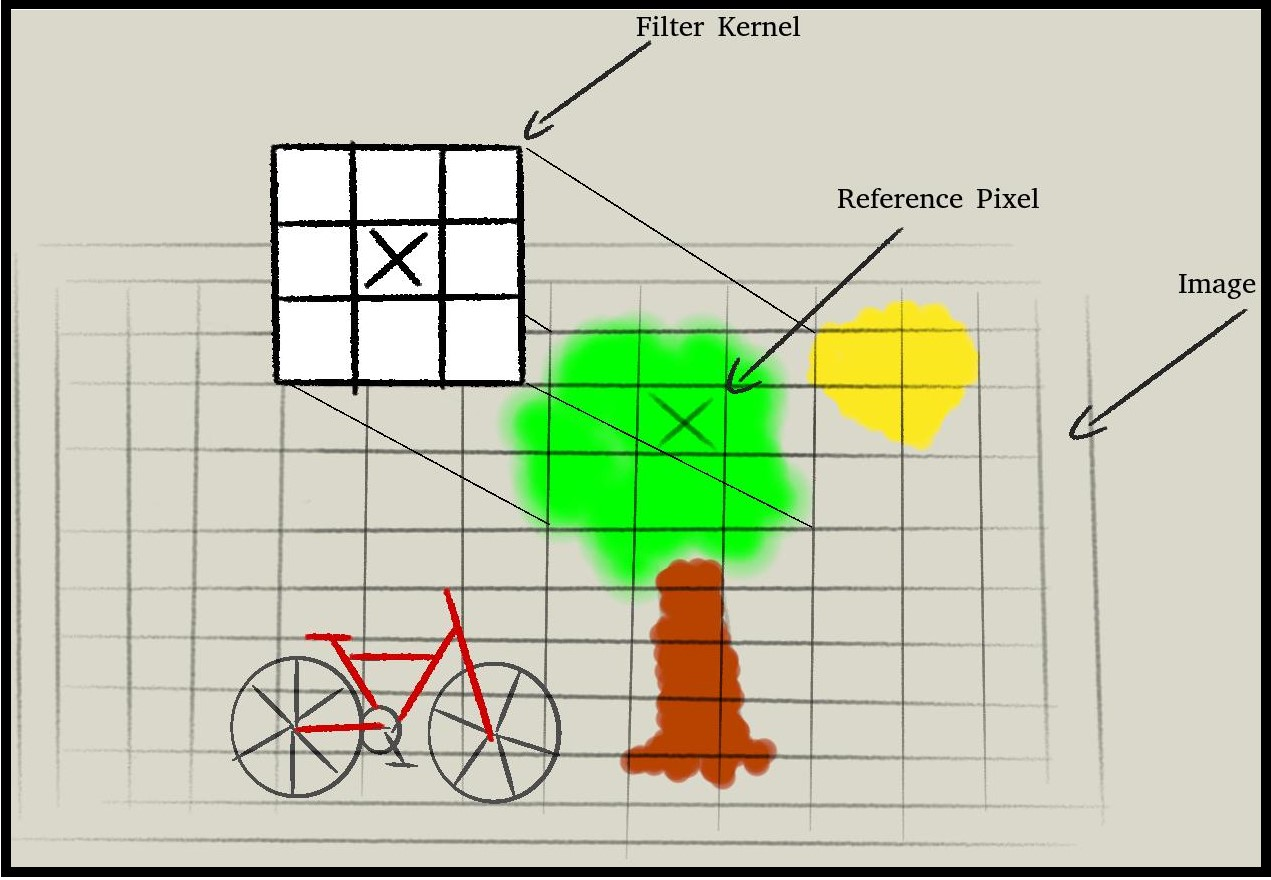
\includegraphics[width=350pt]{kernel_graphics}
  \caption{Visualization of a Filter Kernel Application}
  \label{fig:kernel_graphics}
\end{figure}

A 'box filter', for example, outputs the average of its inputs. This is because the filter weights are evenly distributed. By passing this filter over an image its sharpness is reduced giving a smoothing or blurring effect. This can be observed in Figure \ref{fig:roughDog}.

% DOG BOX FILTERED%
\begin{figure}[H]
  \centering
  \centering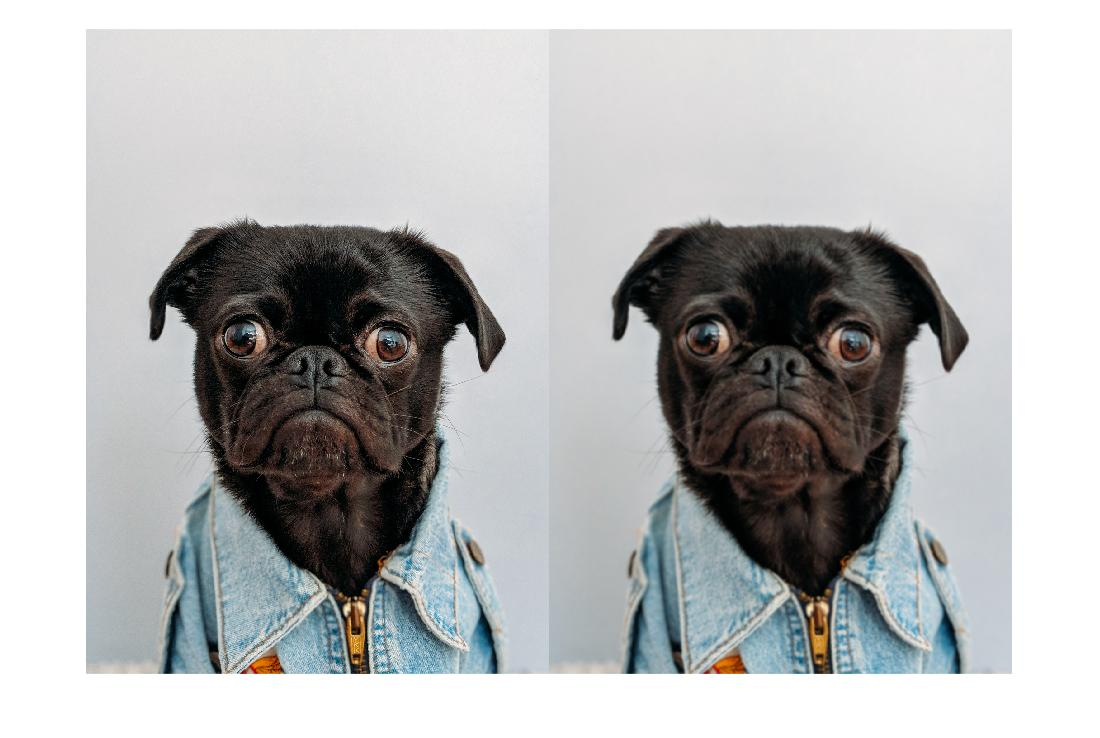
\includegraphics[width=350pt]{dogPug}
  \caption{Left: Photo by Charles Deluvio on Unsplash Right: Application of $16\times16$ box filter.}
  \label{fig:roughDog}
\end{figure}

% CORRELATION
\subsection{Correlation}

The application of a linear filter $h(u,v)$ to an image $f(i,j)$ may be described as follows

\begin{equation} \label{eq:1}
g(i,j) = \sum_{u=-k}^{k}\sum_{v = -l}^{l}f(i+u,j+v)h(u,v)
\end{equation}


The dimensions of the filter kernel are ($2k+1) \times (2l+1$). Filter kernels are nearly always odd dimensioned so as to have a center. This is because an asymmetric kernel, one which has even numbered dimensions, will result in output being distorted \cite{optimalKernel}. This is because the output from the filter will be weighted unevenly by being placed in a reference pixel that is not centered causing aliasing.

% ALIASING
\begin{figure}[H]
  \centering
  \centering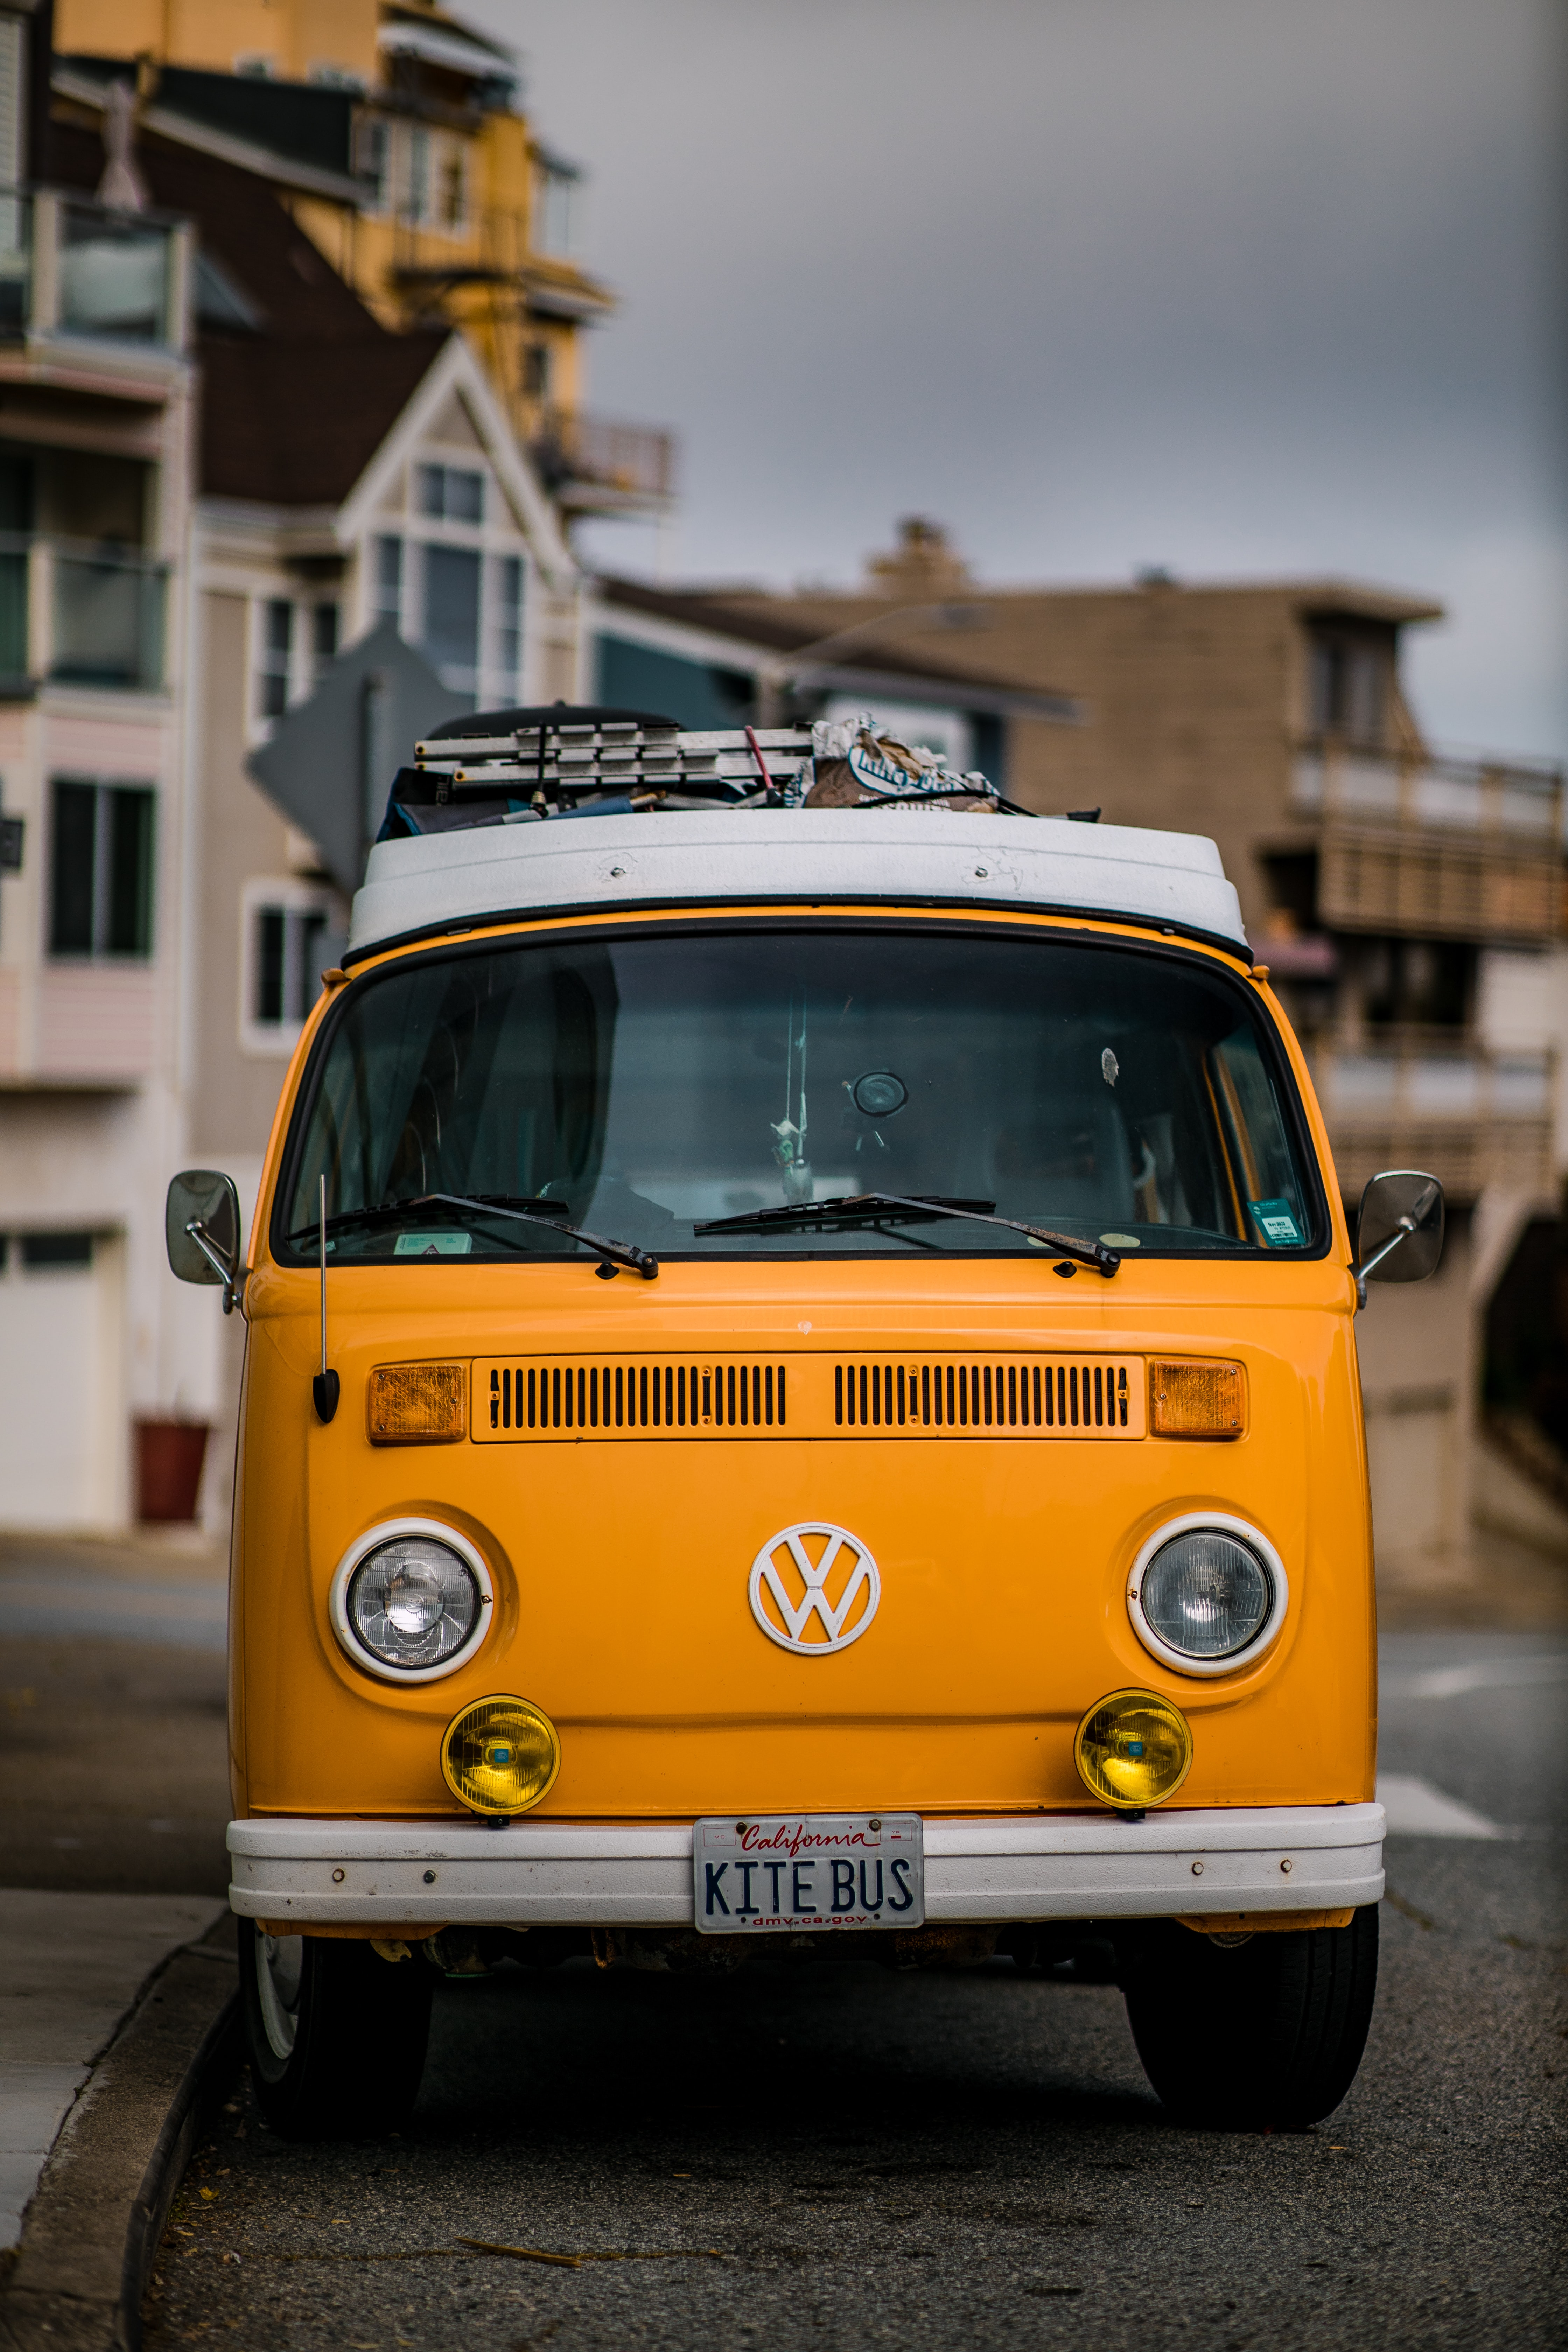
\includegraphics[width=200pt]{van}
  \caption{SHOW IMAGE ALIASING. Photo by Jason Leung on Unsplash}
  \label{fig:van}
\end{figure}

Performing correlation with a filter may be notated more concisely by the \emph{correlation} operator.

\[g = f \otimes h\]

Correlation measures the similarity between two signals. Both digital images and linear filters are two dimensional signals. Performing correlation between them will yield an output image where the highest values correspond to where the image and filter are most similar \cite{optimalKernel}. This useful because if you wish to emphasise a feature in an image it can be done by correlating it with a filter that describes that feature. For example, if you wished to exagerate lines, you could use Sobel filters for vertical and straight lines. These filter masks are composed as in Figure \ref{fig:sobel_filters}.

% SOBEL MASKS
\begin{figure}[H]
  \begin{subfigure}[b]{0.49\textwidth}
    \[
    \begin{bmatrix*}[l]
     -1 & -1 & -1 \\
      \phantom{-}2 & \phantom{-}2 & \phantom{-}2 \\
      -1 & -1 & -1 
    \end{bmatrix*}
    \]
    \caption{Horizontal Sobel Filter Mask}
    \label{rfidtest_xaxis}
\end{subfigure}
\begin{subfigure}[b]{0.49\textwidth}
  \[ 
    \begin{bmatrix}
      -1 & 2 & -1 \\
      -1 & 2 & -1 \\
      -1 & 2 & -1
    \end{bmatrix}
    \]
    \caption{Vertical Sobel Filter Mask}  
\end{subfigure}
    \caption{Sobel Filters}
    \label{fig:sobel_filters}
\end{figure}

Correlation a Sobel filter's, as in Figure \ref{fig:sobel_apply}, isolates the features described by the filter. The filter's are weighted such that if they're sitting atop of line, a high value is produced at that location in the output image. Hence, the output images Figure \ref{fig:vert}, and Figure \ref{fig:hoz} show emphasised vertical and horizontal lines.

% SOBEL FILTER APPLICATION
\begin{figure}[htbp]
  \centering
  \begin{subfigure}[b]{0.3\textwidth}
      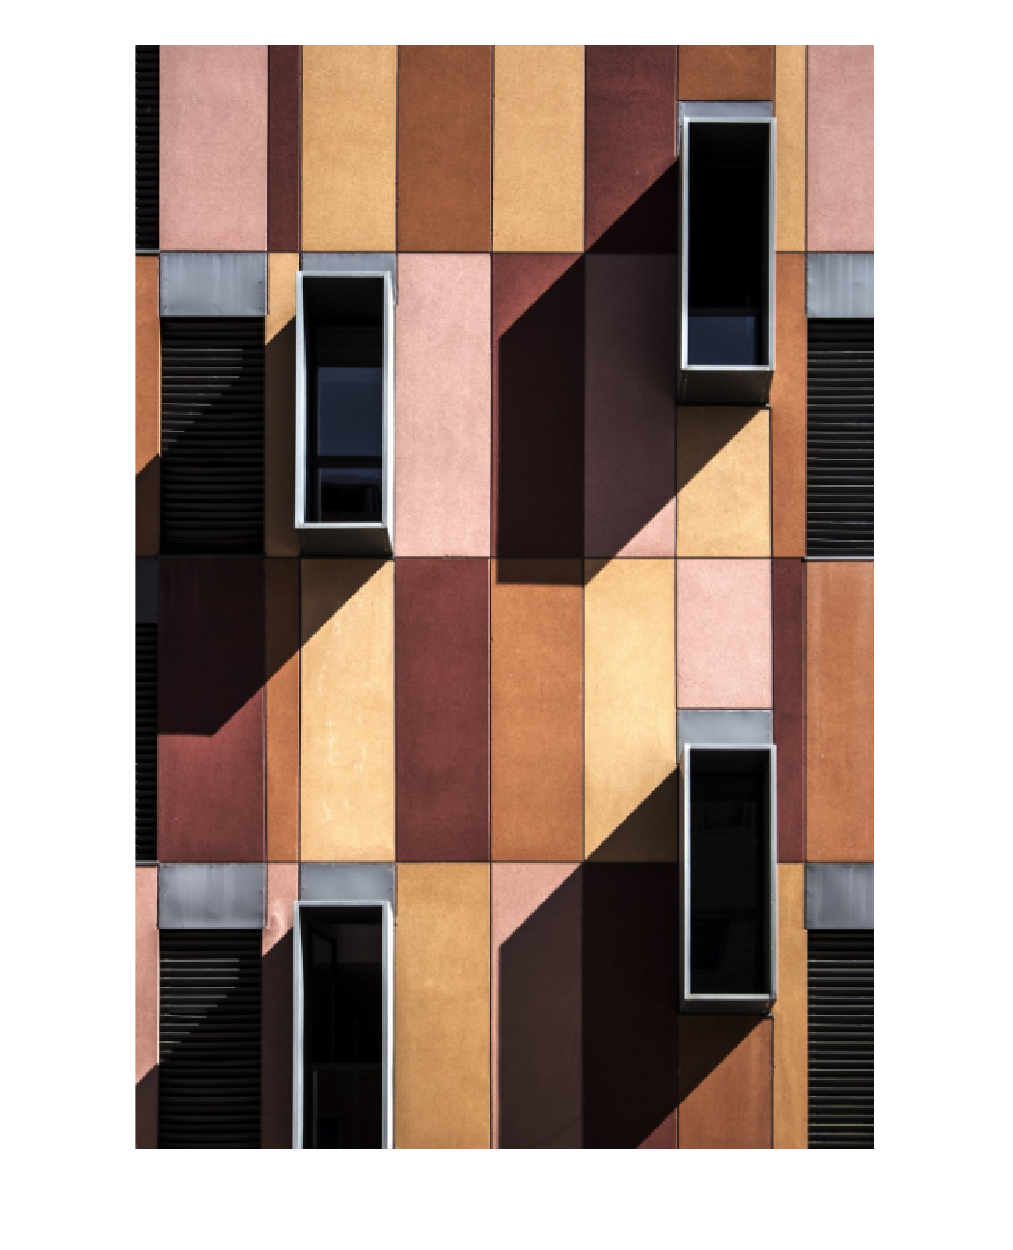
\includegraphics[width=\textwidth]{im_color}
      \caption{Image by Simone Hutsch}
  \end{subfigure}
  \begin{subfigure}[b]{0.3\textwidth}
      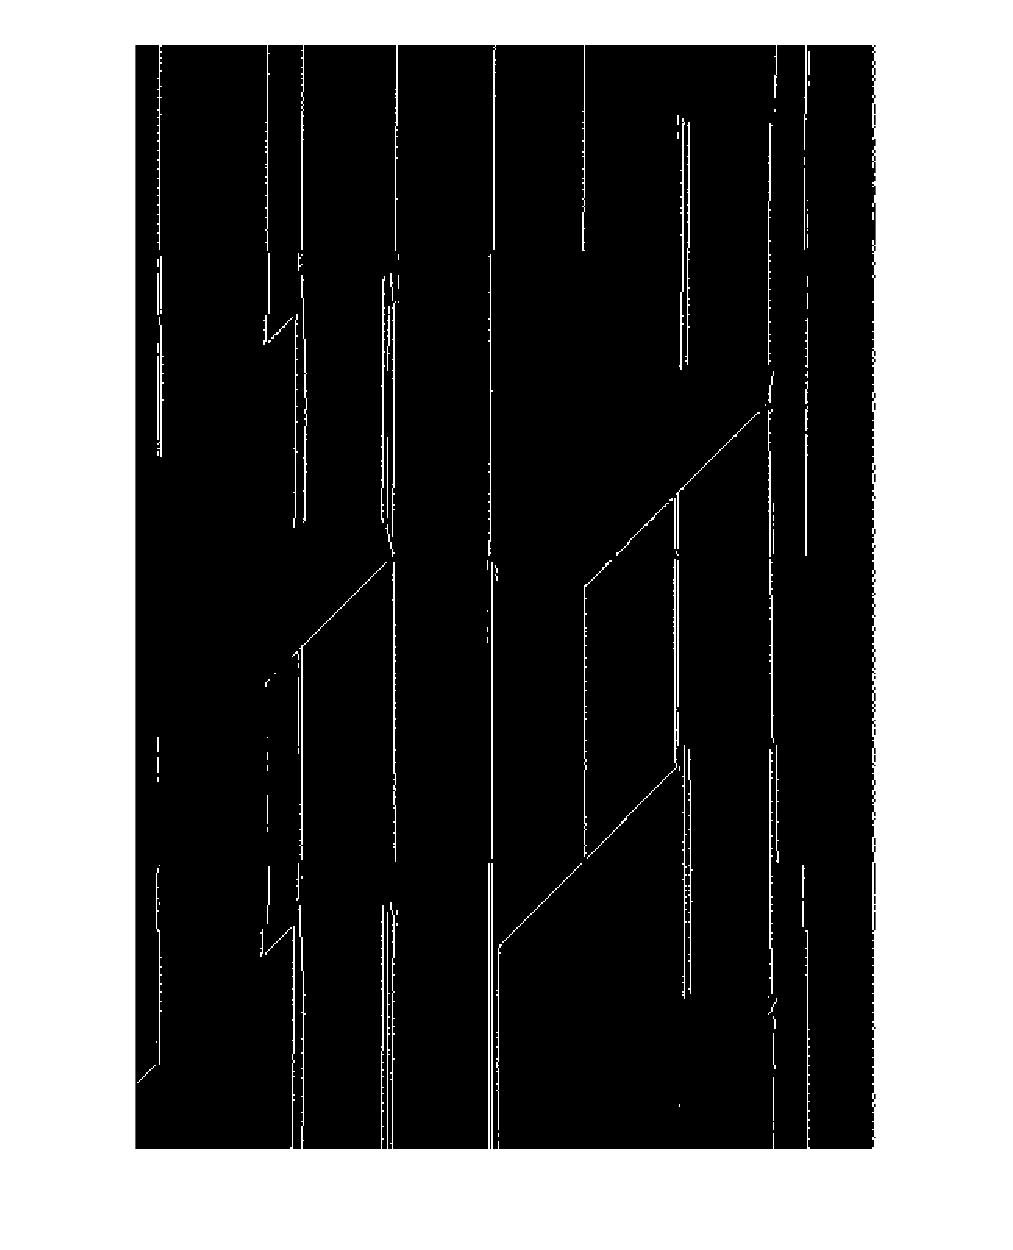
\includegraphics[width=\textwidth]{gv}
      \caption{Vertical Sobel Filter}
      \label{fig:vert}
  \end{subfigure}
  \begin{subfigure}[b]{0.3\textwidth}
      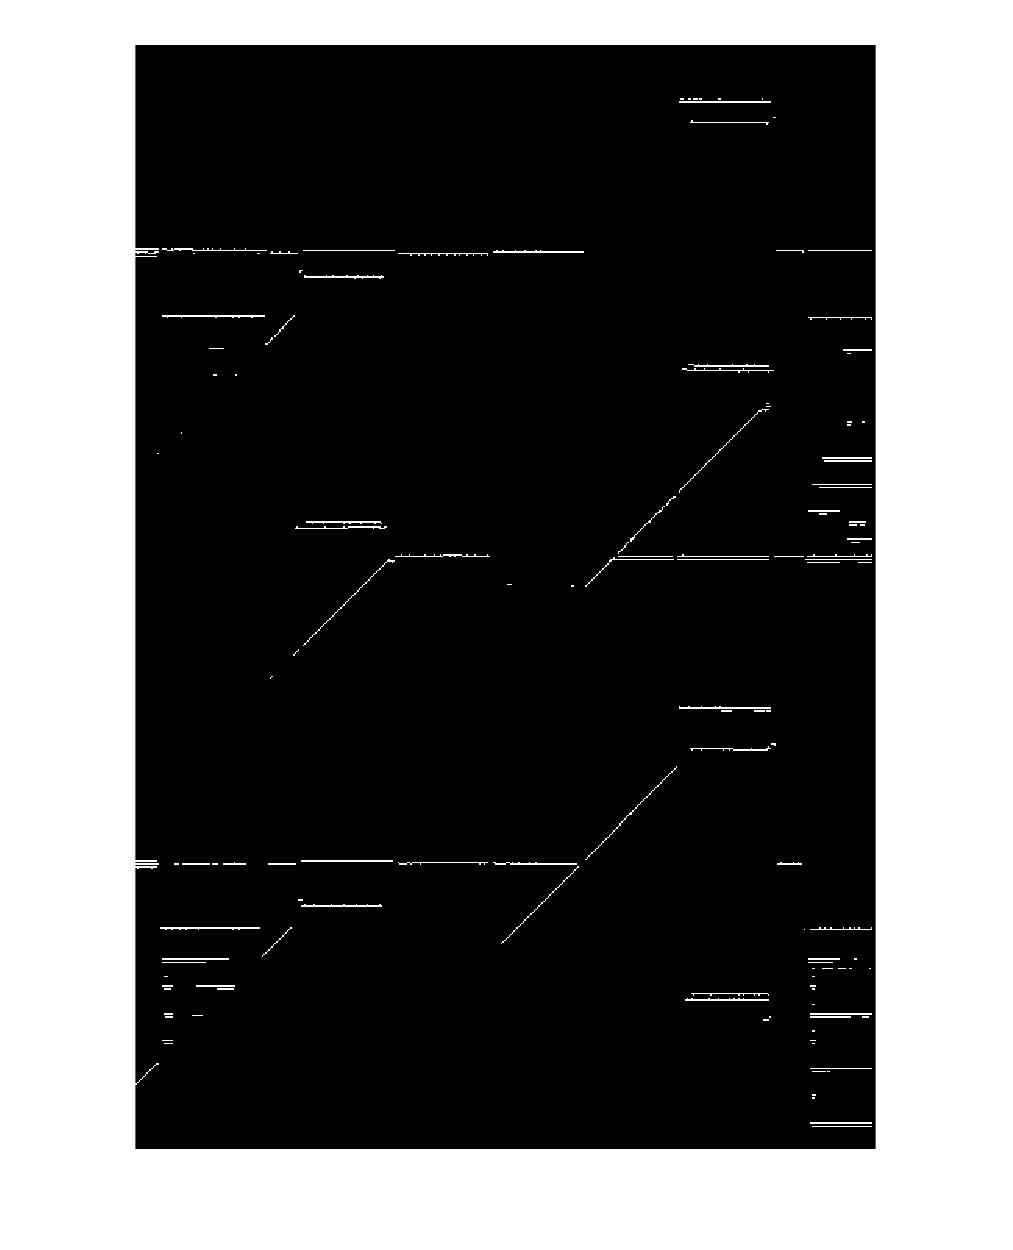
\includegraphics[width=\textwidth]{gh}
      \caption{Horizontal Sobel Filter}
      \label{fig:hoz}
  \end{subfigure}
  \caption{Application of Sobel filters to exagerate lines.}
  \label{fig:sobel_apply}
\end{figure}

Correlation is \emph{shift invariant}, which means that it does the same thing no matter where in an image it is applied. To satisfy this property correlation may be superpositioned 

\[a(f_1 + f_2) = af_1 + af_2\]

and abides by the shift invariance principle

\[g(i,j)=f(i+k,j+l) \Leftrightarrow\ (h\circ g)(i,j)=(h\circ f)(i+k,j+l)\]

Correlation has the side effect of flipping both horizontally and vertically the location of output points relative to location the center point (\emph{reference point}) in the original image which may be undesirable.\newline

% CORRELATION EXAMPLE  %
\begin{figure}[H] 
  \centering
  \begin{tabular}{ccccc}
      \begin{tabular}{|c|c|c|c|c|}
      \hline
      0 & 0 & 0 & 0 & 0 \\[1pt]
      \hline
      0 & 0 & 0 & 0 & 0 \\[1pt]
      \hline
      0 & 0 & 1 & 0 & 0 \\[1pt]
      \hline
      0 & 0 & 0 & 0 & 0 \\[1pt]
      \hline
      0 & 0 & 0 & 0 & 0 \\[1pt]
      \hline
      \end{tabular}%
    & $\otimes$ &
    \begin{tabular}{|c|c|c|}
      \hline
      a & b & c \\
      \hline
      d & e & f \\
      \hline
      g & h & i \\
      \hline 
    \end{tabular}
    & $=$ &
    \begin{tabular}{|c|c|c|c|c|}
      \hline
      0 & 0 & 0 & 0 & 0 \\[1pt]
      \hline
      0 & \textbf{i} & \textbf{h} & \textbf{g} & 0 \\[1pt]
      \hline
      0 & \textbf{f} & \textbf{e} & \textbf{d} & 0 \\[1pt]
      \hline
      0 & \textbf{c} & \textbf{b} & \textbf{a} & 0 \\[1pt]
      \hline
      0 & 0 & 0 & 0 & 0 \\[1pt]
      \hline
    \end{tabular} \\
    $F(x,y)$ & & $H(u,v)$& & $G(x,y)$ \\
  \end{tabular}
  \caption{Correlation of a filter and an image.}
  \label{fig:correlation}
\end{figure}


\subsection{Convolution}

Convolution is also a linear operation that is shift invariant and the order of its operands don't matter. It is very similar to correlation except that where correlation measure similarity between signals convolution measures the effect of one signal on another. It is described mathematically by the expression,

\[ g(i,j) = \sum_{u=-k}^{k}\sum_{v = -l}^{l}f(u,v)h(i-u,j-v)\]

Notice that the filter $h(i,j)$ is rotated  180 degrees. This causes the output's orientation to match the original image.Convolution may be notated as follows,

\[g = f \ast h\]

% CORRELATION EXAMPLE  %
\begin{figure}[H] 
  \centering
  \begin{tabular}{ccccc}
      \begin{tabular}{|c|c|c|c|c|}
      \hline
      0 & 0 & 0 & 0 & 0 \\[1pt]
      \hline
      0 & 0 & 0 & 0 & 0 \\[1pt]
      \hline
      0 & 0 & 1 & 0 & 0 \\[1pt]
      \hline
      0 & 0 & 0 & 0 & 0 \\[1pt]
      \hline
      0 & 0 & 0 & 0 & 0 \\[1pt]
      \hline
      \end{tabular}%
    & $\ast$ &
    \begin{tabular}{|c|c|c|}
      \hline
      a & b & c \\
      \hline
      d & e & f \\
      \hline
      g & h & i \\
      \hline 
    \end{tabular}
    & $=$ &
    \begin{tabular}{|c|c|c|c|c|}
      \hline
      0 & 0 & 0 & 0 & 0 \\[1pt]
      \hline
      0 &  \textbf{a} & \textbf{b} & \textbf{c} & 0 \\[1pt]
      \hline
      0 & \textbf{d} & \textbf{e} & \textbf{f} & 0 \\[1pt]
      \hline
      0 & \textbf{g} & \textbf{h} & \textbf{i} & 0 \\[1pt]
      \hline
      0 & 0 & 0 & 0 & 0 \\[1pt]
      \hline
    \end{tabular} \\
    $F(x,y)$ & & $H(u,v)$& & $G(x,y)$ \\
  \end{tabular}
  \caption{Convolution of a filter and an image.}
  \label{fig:convolution}
\end{figure}